%-------------------------------------------------------------------------------
% LATEX TEMPLATE ARTIKEL
%-------------------------------------------------------------------------------
% Dit template is voor gebruik door studenten van de de bacheloropleiding 
% Informatica van de Universiteit van Amsterdam.
% Voor informatie over schrijfvaardigheden, zie 
%                               https://practicumav.nl/schrijven/index.html
%
%-------------------------------------------------------------------------------
%	PACKAGES EN DOCUMENT CONFIGURATIE
%-------------------------------------------------------------------------------

\documentclass{uva-inf-article}
\usepackage[english]{babel}

\usepackage[
    maxbibnames=10,
    style=authoryear-comp
]{biblatex}
\addbibresource{references.bib}

\usepackage{pdfpages}

%-------------------------------------------------------------------------------
%	GEGEVENS VOOR IN DE TITEL, HEADER EN FOOTER
%-------------------------------------------------------------------------------

% Geef je artikel een logische titel die de inhoud dekt.
\title{The quest to finding the best SNNI}

% Vul de naam van de opdracht in zoals gegeven door de docent en het type 
% opdracht, bijvoorbeeld 'technisch rapport' of 'essay'.
\assignment{Project proposal}
\assignmenttype{}

% Vul de volledige namen van alle auteurs in en de corresponderende UvAnetID's.
\authors{Jorit Prins}
\uvanetids{12862789}

% Vul de naam van je tutor, begeleider (mentor), of docent / vakcoördinator in.
% Vermeld in ieder geval de naam van diegene die het artikel nakijkt!
\supervisors{Zoltan Mann}
% \mentor{Marco Brohet}
\docent{}

% Vul hier de naam van je tutorgroep, werkgroep, of practicumgroep in.
\group{}

% Vul de naam van de cursus in en de cursuscode, te vinden op o.a. DataNose.
\course{Afstudeerproject bachelor Informatica}
\courseid{5062ABI18Y}

% Dit is de datum die op het document komt te staan. Standaard is dat vandaag.
\date{\today}

%-------------------------------------------------------------------------------
%	VOORPAGINA 
%-------------------------------------------------------------------------------

\begin{document}
\maketitle

%-------------------------------------------------------------------------------
%	INHOUDSOPGAVE EN ABSTRACT
%-------------------------------------------------------------------------------
% Niet toevoegen bij een kort artikel, zeg minder dan 10 pagina's!

%TC:ignore
%\tableofcontents
%\begin{abstract}
%\end{abstract}
%TC:endignore

%-------------------------------------------------------------------------------
%	INHOUD
%-------------------------------------------------------------------------------
% Hanteer bij benadering IMRAD: Introduction, Method, Results, Discussion.

%[hebben veelbelovende resultaten en staan aan de voorgrond/voorsprong van] 
\section{Relevance}
The recent rise in Big Data increased the data exchange on the internet. With more and more computer resources available, researchers quickly started to utilise the possibilities of machine learning (ML) to analyse the data.  Techniques like neural networks (NN) are promising ways to scientific breaktroughs. Machine learning has a wide varity of applications for classification such as traffic analysis, image recognition, intrusion detection,  spam detection, medical or genomics predictions,  financial predictions and face recognition \parencite{Dowlin2017, Islam2011, Bachrach16, Kaiming215}

The use of ML typically consists of two phases: training and inference. In the first phase a NN is trained by feeding an extensive dataset to find the best parameters. NNs used for machine learning have to be maintained, evaluated and the training phase is often a tedious and time exhausting process. In the inference phase an input is applied to the trained NN. Because of the time consuming process of creating a NN, machine learning as a service (MLaaS) became popular. In MLaaS, a company offers a pre-trained NN to the clients. Now, clients only need to worry about the inference phase.

However, MLaaS offers great threats to privacy. To train the model as accurately as possible a NN needs access to a large amount of precise data from clients, which may consist of sensitive information. Thus, clients may be reluctant to provide the NNs with their data. Other features, irrelevant to the prediction task, could also be derived from this data \parencite{Nasr2019}. On the inference phase, input from the client to the NN can also be confidential. On the other hand, owners of a NN could be worried that an adversary could steal (parameters of) their (often costly) NN. Furthermore, the result of the NN could also be confidential resulting in the need to retain this information from unauthorized parties. 

A typical MLaaS situation consist of two parties: the client holding an input \textit{x} and a company holding neural network \textit{f}. For this research we will focus on the inferrence part. The client wants to know the applied input \textit{f(x)} while keeping the sensitive contents of \textit{x} and the result \textit{f(x)} private from the company. The company wants to hold the intelectual property \textit{f} private while still giving the opportunity to the client to use \textit{f}. The secure neural network inference (SNNI) problem entails calculating the applied input \textit{f(x)} while still holding all the above security requirements. 

No general implementation of an SNNI has been widely accepted to the authors knowledge. Rapid progress in this area has made it hard to get a good overview of technological advances. Mann et al. (\citeyear{Mann22}) has summarized several proposed approaches for SNNI. However, these approaches are often proof-of-concept and are not thoroughly tested. Moreover, the performance is often only tested on basic measures like efficiency or privacy.

Other metrics like energy concumption, that could be of relevance, are not researched. This could be of importance because limitations on the client side, when a device is battery powered for example or in the case of IoT devices with limited power resources and the overall energy consumption should be low. Companies, on the other hand, also want to keep energy consumption as low as possible because of budget limitations.

\section{Research question(s)}
To contribute to the prior research in this area, I will discuss the energy implications of suggested, open source implementations of SNNIs. A few of these implementations are ABY2.0 \parencite{ABY20}, Chameleon \parencite{Chameleon}, Cheetah \parencite{Cheetah}, CrypTFlow2 \parencite{CrypTFlow2} and Delphi \parencite{Delphi}. The research quesetion is:
\begin{quote} \emph{RQ: What are the energy implications of open source suggestions of SNNIs?} \end{quote} \paragraph{}

To help research the implications of the SNNI, I have defined a subset of research questions:

\begin{quote} \emph{RQa: How do we measure the energy consumption of a SNNI?} \end{quote}
\begin{quote} \emph{RQb: What is the difference between the energy consumption on the client- and  server side and what are the consequences of this difference} \end{quote}

\section{Method}
To answer these aforementioned questions first I will have to select one implementation of a SNNI to start with. Once the implementation is chosen it needs to work on my own setup. Simultanious to this we will answer question \textit{RQa} with an extensive literature search. Once the implementation is set up and we have answered \textit{RQa} we can start testing the implementation.

With the results of this experiment we can answer the first part of \textit{RQb}. The second part of \textit{RQb} can be answered with a literature search. 


\section{Schedule} 
(will come once research questions are formulated good enough => see email)
% 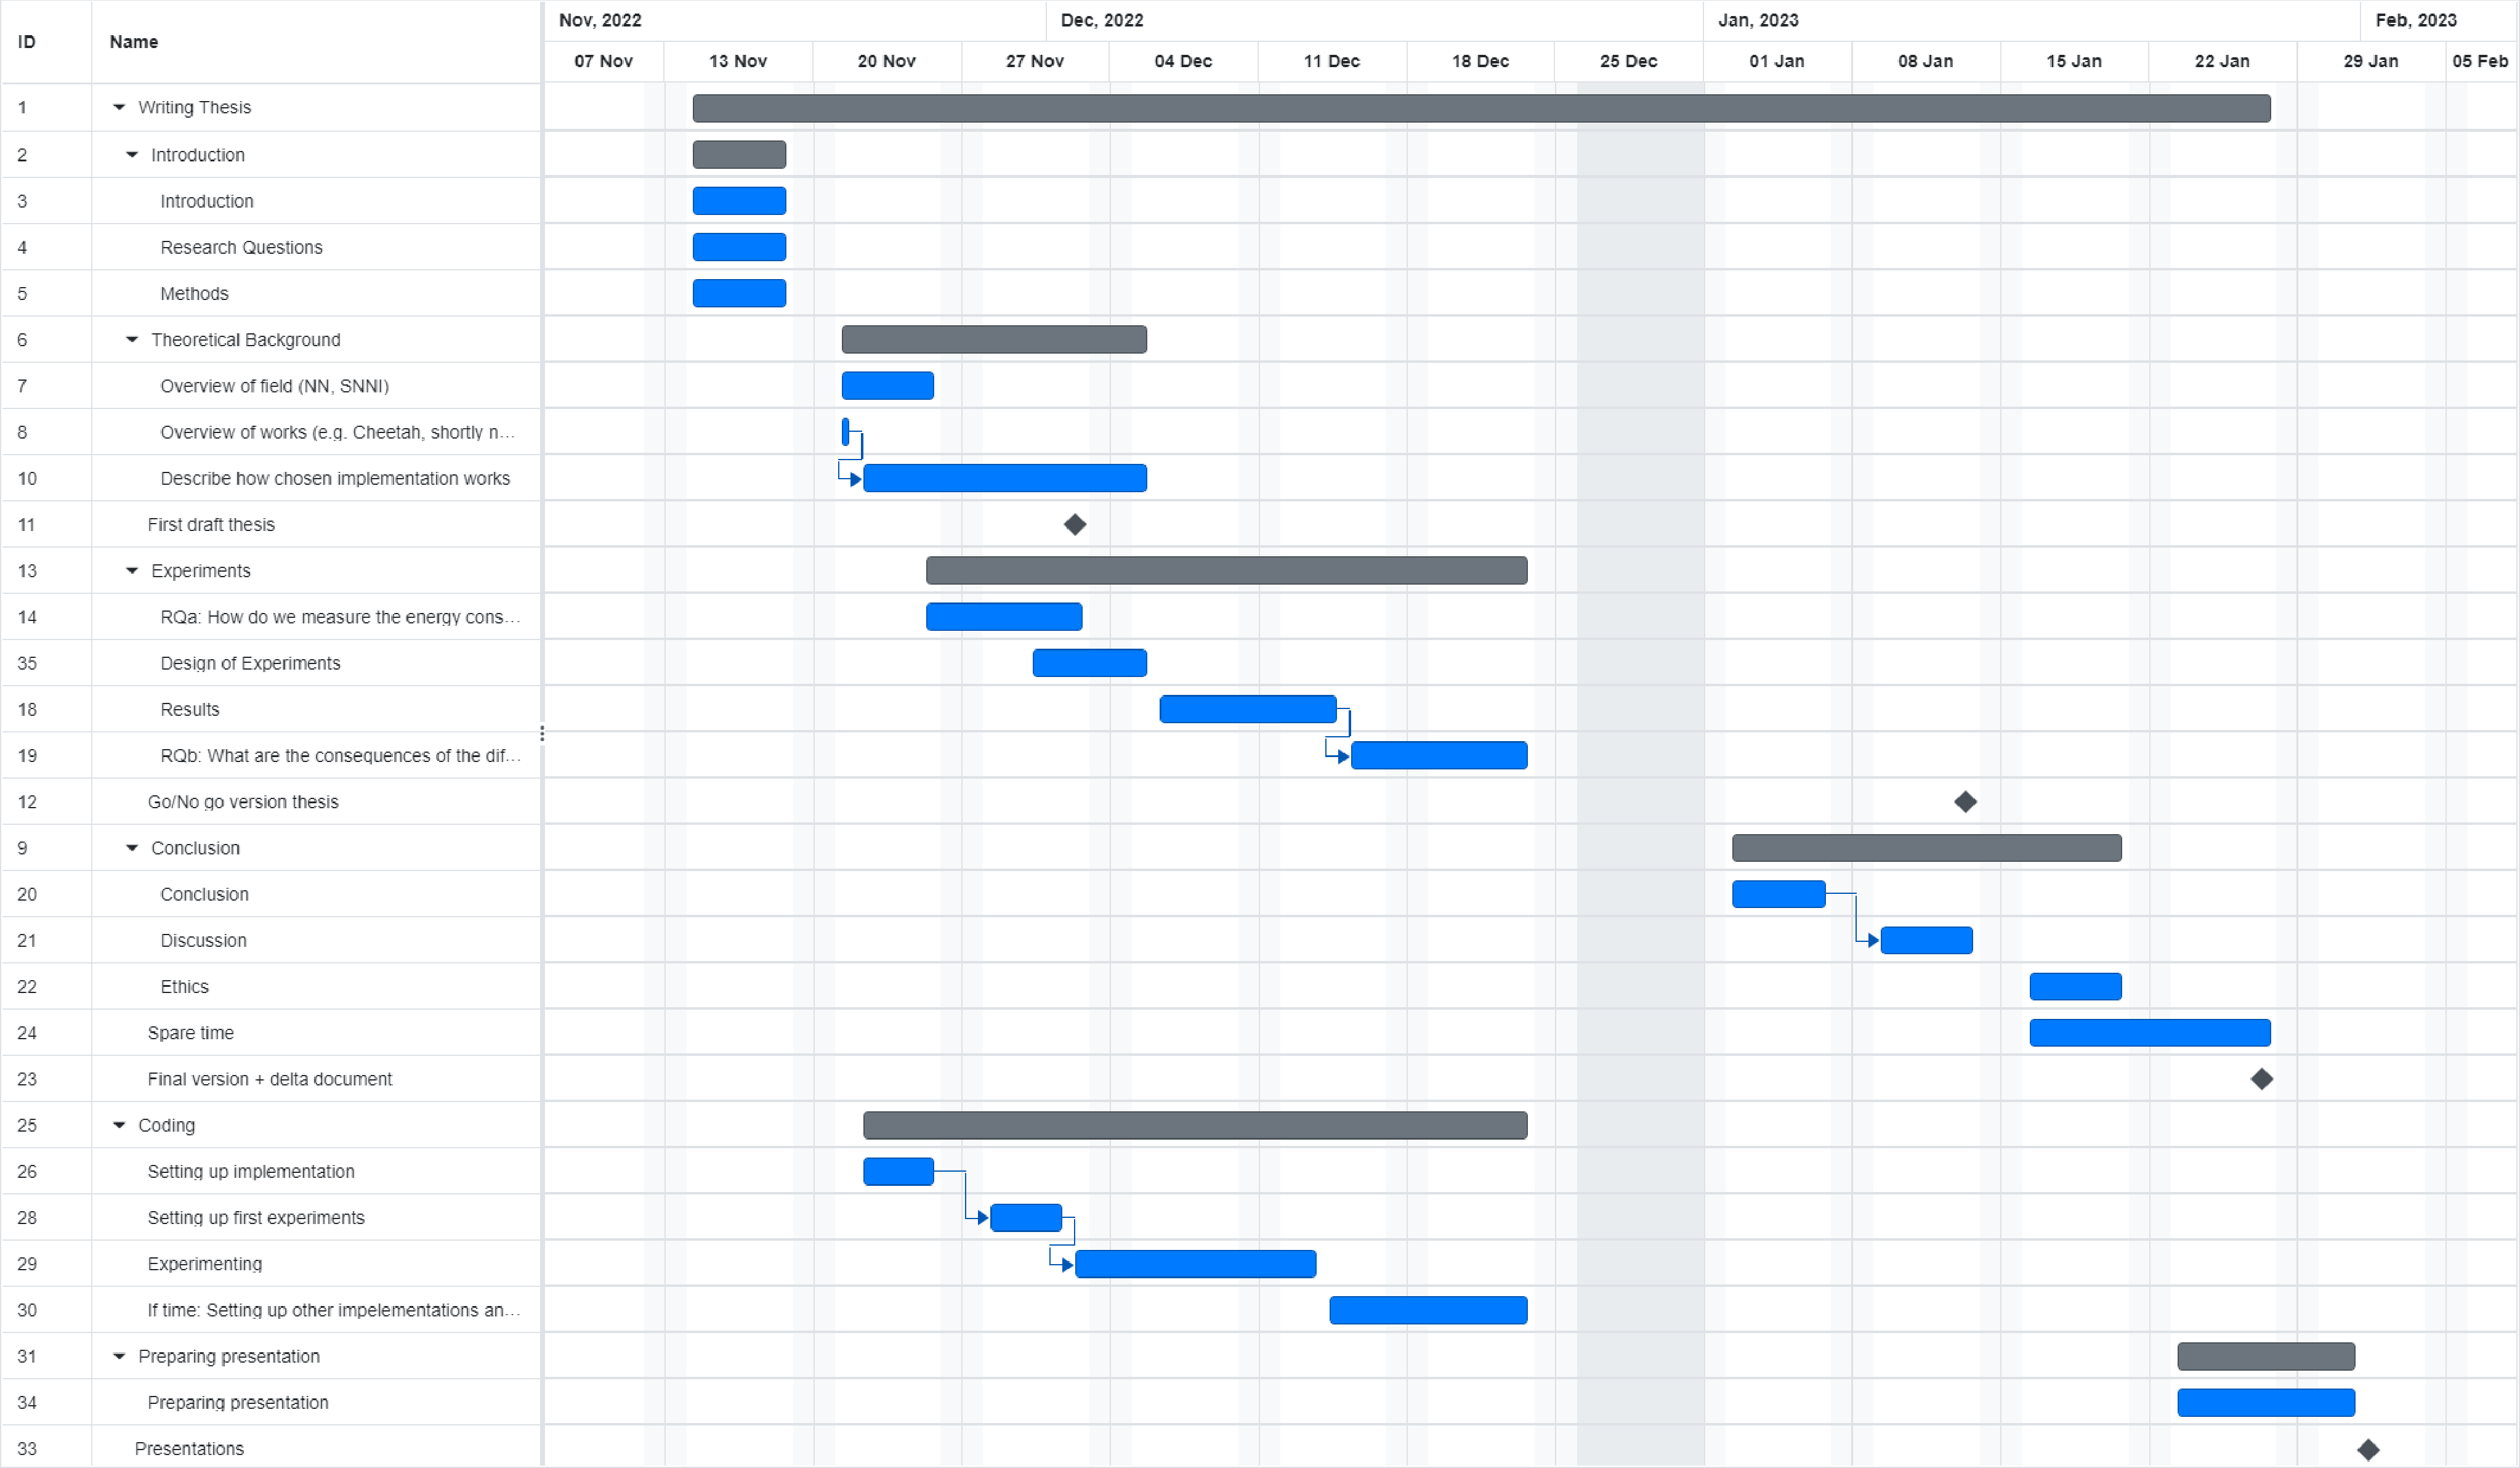
\includepdf[pages=-,angle=270]{Gantchart_Thesis.pdf}


% \subsectionauthor[Voornaam Achternaam]{Paragraaf met auteur}
% \lipsum[2-3]

%-------------------------------------------------------------------------------
%	REFERENTIES
%-------------------------------------------------------------------------------
\newpage
\printbibliography
%-------------------------------------------------------------------------------
\end{document}